\documentclass{article}

\usepackage[utf8]{inputenc}
\usepackage[L7x]{fontenc}
\usepackage[lithuanian]{babel}
\usepackage{lmodern}

\usepackage[many]{tcolorbox}
\usepackage{framed}
\usepackage{mdframed}
\usepackage{animate}
\usepackage{amsmath}
\usepackage{tasks}
\usepackage[top=1.8cm, bottom=1.8cm, left=1.4cm, right=1.4cm, footskip=1cm, a4paper]{geometry}
\usepackage{hyperref}
\usepackage{indentfirst}

\begin{document}
Matematinių taisyklių įrodymas moksleiviams dažniausiai būna per sunkiai suprantamas procesas, todėl prieš daugiau nei 20 metų politiškai buvo nuspręsta, jog mokytis mokyklinių taisyklių įrodymų programoje neprivaloma. Vadovėliuose dauguma taisyklių užrašoma dažniausiai ne tik be įrodymų, bet ir be prasminių (gyvenimiškoms situacijoms pritaikytų) paaiškinimų. Šiuos reiškinius galima pavadinti matematiniu samprotavimo atsisakymu. Iš mokomojo matematinio turinio pašalinus samprotavimą moksleiviai matematiką pradėjo vertinti kaip tarpusavyje nesisiejančių taisyklių ir formulių rinkinį, savo gausa keliantį baimę. Šio straipsnelio motyvas yra kuo paprasčiau apibūdinti ir palyginti praktinę naudą, gaunamą iš prasminių paaiškinimų bei įrodymų nagrinėjimo.
\section*{Ką laikome praktine nauda?}
Praktine nauda šiuo atveju laikome teigiamų veiksnių visumą, nulemiančią aukštą įvertinimą iš matematikos. Pavyzdžiui per kontrolinį išvengtas stresas pasimokius, pakilusi motyvacija žinant, kad pavyko išspręsti sunkiausią uždavinį arba geras taisyklių suvokimas, įgytas dirbant su korepetitoriaus pagalba prieš atsiskaitymą. Vienas iš tokių veiksnių yra kartojimasis prieš mokantis. Jo praktinė nauda yra šitaip aiškinama šiame \href{https://www.pasimokome.lt/2017/12/20/kaip-nepamirsti-ka-ismokai/}{korepetitorių puslapyje}:
\newline
\newline
\edef\myindent{\the\parindent}
{\small{
\fbox{\begin{minipage}[b]{0.49\textwidth}
\setlength{\parindent}{\myindent}
Tikriausiai kiekvienas mokinys ir studentas turėjo atvejų, kai iš karto po kontrolinio, testo ar egzamino išgaruoja visos žinios. Kodėl taip nutinka? Dėl to, jog mokotės paskutinę dieną arba netinkamai išdėliojate mokymosi grafiką. Pažiūrėkite į šią užmiršimo kreivę:
\phantom{xxxxx}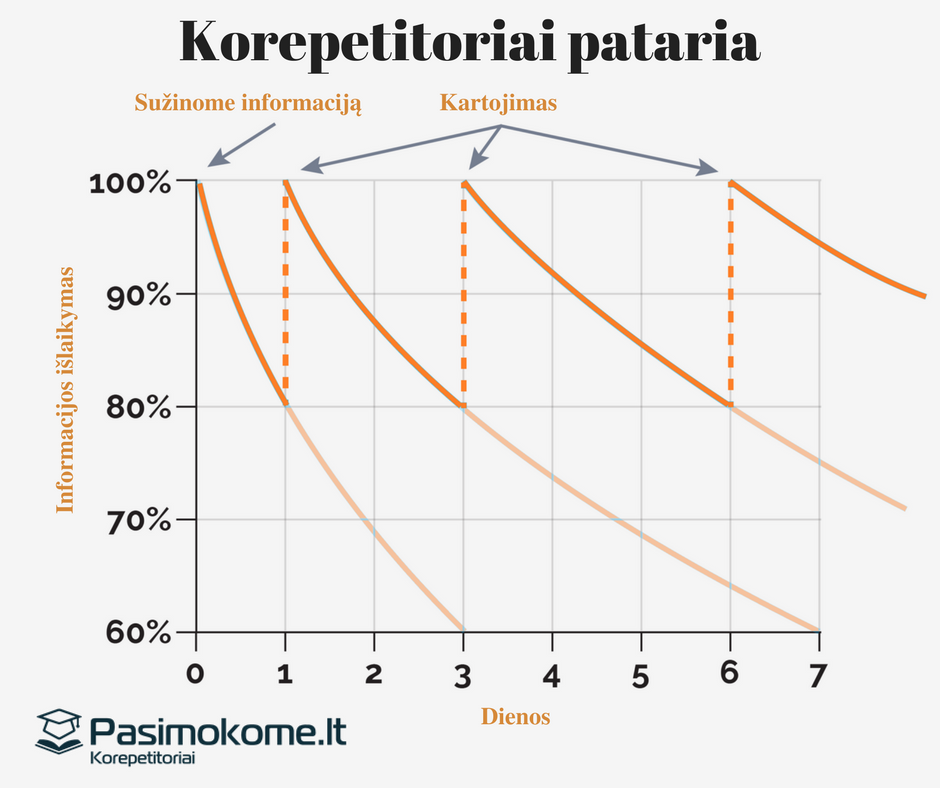
\includegraphics[width=0.7\textwidth]{kartojimas.png}
\end{minipage}}
\hspace{\fill}
\fbox{\begin{minipage}[b]{0.49\textwidth}
\setlength{\parindent}{\myindent}
Tiesa sakant, kreivė atrodo baisiai – vos tik išmokstame informaciją, jau kitą dieną labai daug pamirštame. Tačiau grafikas atrodo daug geriau, kai mokymasis yra suskirstytas į intervalus ir medžiagą mes pasikartojame kas tam tikrą laiką.

Tai kaip galima mokytis ir viską atsiminti net ir po mėnesio, metų ir ilgiau? Kartojimas yra mokslų motina. Tikriausiai pagalvojote „Ačiū, nežinojome“. Tačiau tikrai nedidelė mokinių ir studentų dalis taiko šį metodą.

Jūs žymiai lengviau atsiminsite informaciją, jei ją kartosite intervalais. Įsiminę informaciją, ją pakartokite kitą dieną. Po to vėl ją pakartokite po 3 dienų, vėliau – po savaitės. Kartojant informaciją intervalais, ji išsisaugo žymiai ilgesniam laikui. Mokydamiesi tokiu būdu, išvengsite tokių situacijų, kai po egzamino ar kontrolinio iš karto pasimiršta visa informacija. Tam, jog būtų paprasčiau naudoti šį metodą, savo telefono kalendoriuje pasižymėkite dienas ir laikus, kada turite pasikartoti medžiagą. Taip tikrai nepamiršite pasikartoti.

Tačiau žinoti neužtenka – būtinai taikykite šį metodą praktikoje.
\end{minipage}}}}

Nors būtų neteisinga prieštarauti, jog kartojantis rezultatai pagerėja, tačiau tai nepaaiškina, kodėl kai kurie moksleiviai intensyviai kartodamiesi negali pasiekti tokių aukštų rezultatų kaip gabesnieji, dažnai įdedantys mažiau pastangų. Dažnai gabesnieji moksleiviai kur kas geriau nujaučia tai, ką reikia įsiminti per matematikos pamokas, kad įsimintą informaciją pavyktų sėkmingai atkurti per atsiskaitymus.

Šiame straipsnelyje pagrindiniu praktinės naudos veiksniu laikysime galimybes kuo geriau matematinėje medžiagoje atrinkti tai, ką įsiminti, kad įsimintą medžiagą galima būtų kuo geriau atkurti per atsiskaitymą.

\section*{Taisyklės}
Įsivaizduokite, kad esate 7 klasėje ir stengiatės kuo geriau įsiminti veiksmus su neigiamais ir teigiamais skaičiais. Mokymosi sunkumai, su kuriais susidursite, greičiausiai atsikartos ir kitose temose. Pervertus visą skyrių, iš kurio rašomas kontrolinis, atrasite daug taisyklių, kaip pavyzdžiui:
\begin{itemize}
\item \textit{Sudėdami skaičius su vienodais ženklais: parašome bendrąjį dėmenų ženklą ir sudedame tų skaičių modulius.}
\item \textit{Kai abu dauginamieji yra skirtingų ženklų, tai jų sandauga neigiama.}
\end{itemize}

Tai, ką jūs darote klasės darbo metu, greičiausiai bus nuolatinis veiksmų su neigiamais ir teigiamais skaičiais kartojimas tol, kol išmoksite nesunkiai spręsti daug veiksmų reikalaujančius uždavinius, tokius kaip $\left(-3\frac{1}{2}: 1,75\right)+1,1$. Toks mokymasis ilgainiui gali tapti nuobodus, o įgyta patirtis yra neprasminga, nepatikrinama ir slopinanti tolimesnį norą mokytis. Atėjus kontroliniui kai kurie moksleiviai negeba atlikti veiksmų, tokių kaip $-2,5+3$ arba $40:(-5)$, nes nežinojo būdų, kaip įsiminti tiek daug taisyklių, jų nesuprato, arba per mažai kartojosi. Net ir išmokus neigiamų ir teigiamų skaičių veiksmų taisykles, jos dažnai užsimiršinėja.

\newpage
\section*{Taisyklių prasminiai paaiškinimai}
Išeitis iš minėtos keblios situacijos galėtų būti mokymasis naudojant prasminius paaiškinimus. 

\begin{mdframed}[backgroundcolor=yellow!50!white]
Prasminis paaiškinimas - tai toks taisyklės paaiškinimas, kuomet kiekvienam skaičiui, aritmetiniui veiksmui ar kitas matematiniam elementui yra suteikiama neprieštaringa prasmė iš mus supančio pasaulio.
\end{mdframed}

Prasminio paaiškinimo pavyzdys:

\begin{tabular}{|c|l|}
\hline
\textbf{Veiksmas} & \textbf{Prasmė} \\ \hline 
$2 - 3,5 = -1,5$ & uždirbau 2 ir išleidau 3,5, vadinasi turiu 1,5 minuso\\ \hline
$-1,5 - 3,5 = -5$ & išleidau 1,5 ir išleidau 3,5, vadinasi turiu 5 minuso\\ \hline
$-1,5 + 3,5 = 2$ & išleidau 1,5 ir uždirbau 3,5, dabar turiu 2 pliuso\\ \hline
$-1,5 -(- 3,5) = 2$ & išleidau 1,5 ir  {\color{red}išleidau išleidau} 3,5, dabar turiu (?) \\ \hline
\end{tabular}

Iš paskutinio veiksmo pavyzdžio matome, kad ne visada prasminis paaiškinimas yra pakankamai stiprus paaiškinti visiems veiksmams. Tai yra dažnas atvejis matematikoje pereinant prie vis sudėtingėjančių sąvokų. Nepaisant to reiktų (kiek pavyksta) išlaikyti kūrybiškumą ir paieškoti naujų prasmių:

 \begin{tabular}{|c|l|}
\hline
\textbf{Veiksmas} & \textbf{Prasmė} \\ \hline 
$2 - 3,5 = -1,5$ & pirmyn 2 ir atbulai 3,5, vadinasi atbulai 1,5\\ \hline
$-1,5 - 3,5 = 5$ & atbulai 1,5 ir atbulai 3,5, vadinasi atbulai 5 \\ \hline
$-1,5 + 3,5 = 2$ & atbulai 1,5 ir pirmyn 3,5, vadinasi pirmyn 2\\ \hline
$-1,5 -(- 3,5) = 2$ & $\begin{array}{ll}\text{atbulai 1,5 ir  {\color{teal}atbulai nuo atbulinės krypties 3,5,}}\\ \text{ vadinasi atbulai 1,5 ir pirmyn 3,5, vadinasi pirmyn 2} \end{array}$ \\ \hline
\end{tabular}

Iš šių pavyzdžių reikia prisiminti tik tiek, kad skaičių sudėtį ir atimtį lengviausia paaiškinti suteikiant veiksmams tokias prasmes: 
$$\text{Skaičius} = \begin{cases} \text{\textbf{poslinkis pirmyn}, jei jis teigiamas} \\ \text{\textbf{poslinkis atgal}, jei jis neigiamas}\end{cases} \text{Minuso ženklas} = \text{\textbf{krypties apgręžimas}}$$

Taip pat matėme, kad sudėties ir atimties prasmė gali būti $$\text{Skaičius}=\begin{cases} \text{\textbf{uždirbta suma}, jei skaičius teigiamas} \\ \text{\textbf{išleista suma}, jei skaičius neigiamas}\end{cases},$$ tačiau ji nepakankamai užbaigta, nes išleistos sumos apgręžimas sunkiai interpretuojamas.

Panašiomis idėjomis remdamiesi galime sugalvoti, kokią prasmę turi teigiamų ir neigiamų skaičių daugyba.

\begin{tabular}{|c|l|}
\hline
\textbf{Veiksmas} & \textbf{Prasmė} \\ \hline 
$2 \cdot 3,5 = 7$ & 2 kartus sutikau uždirbti po 3,5, vadinasi turiu 7 pliuso\\ \hline
$2 \cdot (-3,5) = -7$ & 2 kartus sutikau išleisti po 3,5, vadinasi turiu 7 minuso\\ \hline
$-2 \cdot 3,5 = -7$ & 2 kartus atsisakiau uždirbti po 3,5, vadinasi turiu 7 minuso\\ \hline
$-2\cdot (- 3,5) = 7$ & 2 kartus atsisakiau išleisti po 3,5, vadinasi turiu 7 pliuso \\ \hline
\end{tabular}

Šiuo atveju daugybos prasmė tokia:

$$\text{Pirmas daugiklis} = \begin{cases} \text{\textbf{kiek kartų sutikau}, jei jis teigiamas} \\ \text{\textbf{kiek kartų atsisakiau}, jei jis neigiamas}\end{cases}$$ $$\text{Antras daugiklis} = \begin{cases} \text{\textbf{uždirbta suma}, jei jis teigiamas} \\ \text{\textbf{išleista suma}, jei jis neigiamas}\end{cases}$$

\section*{Teoremų įrodymai}
\begin{mdframed}[backgroundcolor=yellow!50!white]
Matematinis įrodymas - tai toks taisyklės aiškinimas, kuriame faktai grindžiami tik matematinėmis aksiomomis (akivaizdžiais teiginiais) arba jau įrodytomis taisyklėmis.
\end{mdframed}

Norėdami pamatyti bent vieno matematinio įrodymo pavyzdį panagrinėkime Pitagoro teoremos įrodymo žinsnius. 

Pitagoro teorema teigia, kad jei stačiojo kraštinio statiniai lygūs $a$ ir $b$, o įžambinė lygi $c$, tai $a^2+b^2=c^2$. Vienas iš būdų įrodyti šį teiginį yra nagrinėti brėžinyje pateiktą geometrinę konstrukciją, kurioje pavaizduotas įbrėžtas į kvadratą keturkampis taip, kad jo kvadrato kraštines jis dalytų į kraštines, kurių ilgiai yra $a$ ir $b$.
\newpage
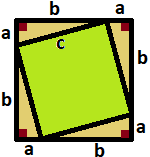
\includegraphics[width=0.15\textwidth]{pyth.png}
\begin{enumerate}
\item Pagal trikampių lygumo požymius visi brėžinyje esantys trikampiai yra lygūs.
\item Pagal trikampių lygumą įbrėžto keturkampio kraštinės lygios.
\item Pagal trikampių lygumą visi įbrėžto keturkampio kampai yra gaunami vienodai (atimant iš $180^o$ po vienodą smailiųjų kampų porą.
\item Pagal kvadrato apibrėžimą kturkampis, kurio kampai vienodi ir kraštinės vienodos, yra kvadratas.
\item Pagal trikampio ploto formulę trikampio plotas lygus $\frac{ab}{2}$. Vadinasi 4 trikampių plotai lygus $2ab$. 
\item Pagal kvadrato ploto formulę įbrėžto kvadrato plotas lygus $c^2$.
\item Didesniojo kvadrato plotas lygus šių plotų sumai $2ab+c^2$
\item Iš kitos pusės didesniojo kvadrato kraštinės ilgis lygus $a+b$, taigi jo plotas taip pat lygus $(a+b)^2$.
\item Prilyginame: $(a+b)^2=2ab+c^2$
\item Pagal kvadratų skirtumo formulę lygybėje pakeičiame kairę pusę: $a^2+2ab+b^2=2ab+c^2$
\item Abejose lygybės pusėse pašalinę dėmenį $2ab$ gauname tai, ką reikėjo: $a^2+b^2=c^2$.
\end{enumerate}

Pitagoro teoremos įrodymas susideda tik iš tokių žingsnių, kuriuos galima paaiškinti remiantis mokykline programa ligi 8 klasės. Vadinasi Pitagoro teoremos įrodymą galima suprasti baigus 8 klases. Norėdami pavaizduoti šių žingsnių tarpusavio ryšį Pitagoro teoremos įrodymą pavaizduosime tokia schema:

\noindent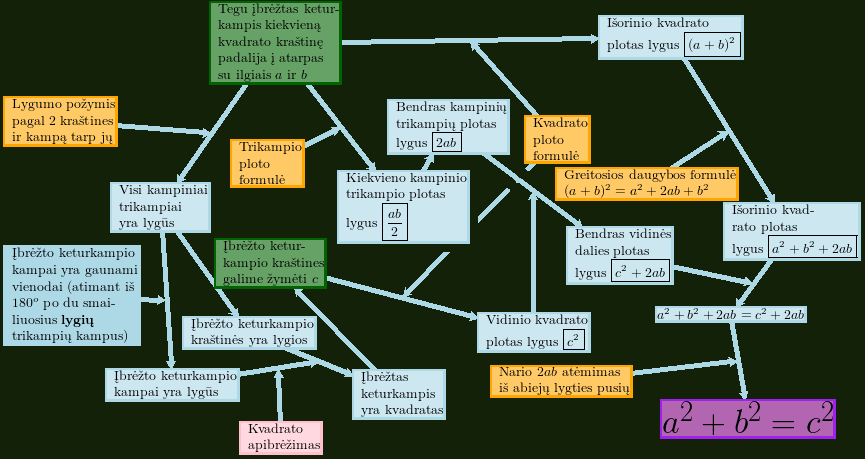
\includegraphics[width=\textwidth]{pythagorian_schema.png}

Keletas paaiškinimų dėl sutartinių žymėjimų:

\begin{itemize}
\item Atskiri įrodymo žingsniai žymimi šviesiai mėlyna spalva.
\item Oranžine arba rožine spalva žymimos mokyklinės taisylės, kurias reikia taikyti norint atlikti žingsnius.
\item Žalia spalva žymimos įvedamos sąlygos
\item Violetine spalva žymimas iš jų išvestas teiginys.
\item Rodyklė tarp dviejų blokų žymi loginį žingsnį, o į ją nukreipta kita rodyklė žymi jo paaiškinimą.
\end{itemize}

Iš pirmo žvilgsnio gali atrodyti, jog šis matematinis įrodymas savyje talpina tiek faktinės medžiagos, jog gali būti įdomus tik matematikos mėgėjams. Daugumą į mokyklinę programą įtrauktų taisyklių galima įrodyti matematiškai arba jos yra matematinės aksiomos. Nesudėtingi įrodymai dažniausiai susideda iš keleto žingsnių, kurie remiasi taisyklėmis, įeinančiomis į mokyklinę programą, tačiau moksleiviui gali būti arba lengvesni, arba užtrunkantys suprasti. Sudėtingesni įrodymai (pvz. išvestinių ir integralų taisyklės) gali susidėti iš tokių žingsnių, kurių supratimas moksleiviui nėra prieinamas, nes jis nestudijuoja aukštosios matematikos. 

Tačiau turėtų kilti klausimas, ar supratimu laikome gebėjimą paaiškinti kiekvieną įrodymo žingsnį, ar tik pritaikyti, o gal visus žingsnius reiktų atsiminti iš eilės? Mokyklinėje programoje didžiausias dėmesys skiriamas tik taikymui (be paaiškinimų kodėl žingsnis gali būti pritaikytas įrodyme). Žingsnių paaiškinimas yra gera priemonė pasitikrinti, kiek mūsų supratime yra logika paremto taisyklių taikymo ir kiek nuo logikos atriboto įsitikinimo, jog mūsų uždavinio sprendimas yra geras.

Žingsnių paaiškinimas turi ir kitą paskirtį: atminties prasme jie yra tarsi medžiaga, kuri sulipdo padrikai taikomas taisykles.
Didėjant matematiniams gebėjimams žinios galvoje mums nejuntant persiformuoja taip, kad atliekami procesai, į kuriuos įeina tos pačios pasikartojančių žingsnių sekos, atmintyje nusistovėtų kaip vientisesni daug atminties nereikalaujantys objektai. Tai paaiškina, kodėl moksleivio gabumai didėja, jei jis bent keletą kartų atlieka panašius samprotavimus. Toks moksleivis, norėdamas sumąstyti pažingsniui sprendžiamo uždavinio sprendimą, jau gali nebesistengti ieškoti užuominų sunkiai prisimenamose taisyklėse, o vietoj to jas ima taikyti savaime nesunaudodamas didesnių atminties resursų. Dabar Pitagoro teoremos įrodymo eiga jam galėtų atrodyti paprastesnė:
\newline
\newline
\noindent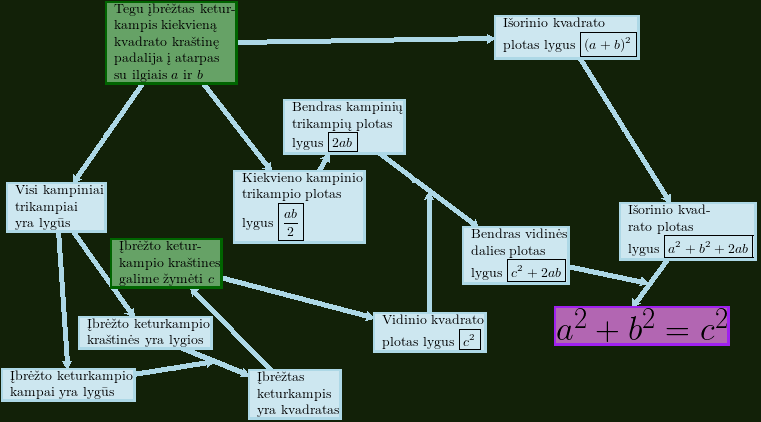
\includegraphics[width=0.95\textwidth]{pythagorian_restructure.png}

Moksleiviai, besidomintys matematika už mokyklos ribų, savo mąstymo lankstumą gali dar labiau padidinti. Vaizdžiai tariant bet kuris moksleivis mokydamasis matematiką stimuliuoja jungtis tarp neuronų. Biocheminių pokyčių pagalba intensyviausiai stimuliuojamos jungtys tampa aktyviausiomis, todėl tam tikri mąstymo keliai tampa vis labiau susiekti. Dėl šių neuroprocesų jūsų matematinis supratimas gali būti vystomas be ribų. Pateiksime paskutinį Pitagoro teoremos išvedimo mintinį žemėlapį, kurį mintyse gali turėti puikiai matematiškai mąstyti gebantys moksleiviai:
\newline
\newline
\noindent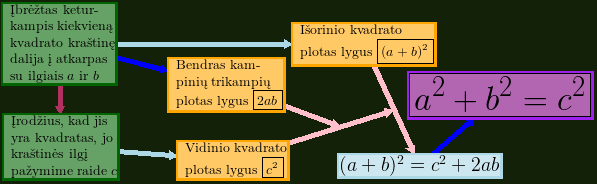
\includegraphics[width=\textwidth]{pythagorian_finalform.png}
Pabaigai atkreipsime dėmesį, kad oranžine spalva nuspalvinti blokai pagal įsimenamos infomacijos pobūdį buvo labai panašūs. Tuo pasinaudodami apibūdinsime, koks Pitagoro teoremos vaizdinys yra matematiko Simono galvoje:

\begin{mdframed}[backgroundcolor=yellow!50!white]
Pitagoro teorema - tai išvada, kurią gauname geometrinėje konstrukcijoje \raisebox{-3.8ex}{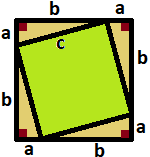
\includegraphics[width=0.07\textwidth]{pyth.png}} dviem skirtingais būdais suskaičiuodami didesniojo kvadrato plotą.
\end{mdframed}

Simonas giriasi, jog svarbiausia, ką jis atsimena apie Pitagoro teoremos išvedimą, yra tik pavaizduota nesudėtinga geometrinė konstrukcija, o visą likusią įrodymo eigą jis gali atkurti vien panaudodamas savo bendrą matematikos išsilavinimą.

\section*{Prasminiai paaiškinimai vs teoremų įrodymai: praktinė nauda}

Priminsime, jog šiame straipsnelyje praktinės naudos veiksniu laikome galimybes kuo produktyviau atkurti išmoktą medžiagą atsiskaitymo metu. Skyrelyje \textbf{Taisyklės} buvo iškelta problema, jog mokantis per atsiskaitymus (ypač sprendžiant daugiau veiksmų reikalaujančius uždavinius) taisyklės dažnai užsimiršta. Susidūrus su nauja taisykle reikėtų neskubėti jos kalti mintinai, o pamėginti sugalvoti jai prasminį paaiškinimą. Prasminius paaiškinimus dažnai atsiminti būna daug lengviau nei taisykles. Jei ruošdamiesi atsiskaitymui arba per atsiskaitymą taisyklę pamiršote, pabandykite ją atkurti panaudodami prasminį paaiškinimą. Remiantis Simono patirtimi užtenka tik keleto to paties prasminio paaiškinimo panaudojimų, kad taikoma taisyklė atmintyje taptų neišblėstanti, o prasminiai paaiškinimai būtų nebūtini. Jie yra tarsi statybinė medžiaga, skirta įtvirtinti taisykles visam laikui. Kiekvienas moksleivis savo mintyse konstruoja savo vidinę matematiką, kuri yra sutvirtinama teisingais ir klaidingais prasminiais paaiškinimais arba paaiškinimais, kurie nėra prasminiai. Taigi matematinį supratimą šiuo atveju galima laikyti tarsi statiniu, kurio tvirtumas priklauso nuo statybinės medžiagos.

Teoremų įrodymas turi kitokią paskirtį. Dažniausiai jis kaip produktyvus taisyklės atkūrimas atmintyje netinka. Pavyzdžiui atsiminti lygybę $a^2+b^2=c^2$ yra daug paprasčiau, nei panaudoti Pitagoro teoremos įrodymą tam, kad šią formulę galėtume atkurti. Tačiau Pitagoro teoremos sandaroje matėme daugybę paprastesnių taisyklių, kuriomis rėmėmės nagrinėdami įrodymo žingsnius. Pirmoji įrodymo schema pakankamai aiškiai jas pateikia:
\begin{itemize}
\item Trikampių lygumo požymis pagal 2 kraštines ir kampą tarp jų
\item Trikapio ploto formulė
\item Kvadrato ploto formulė
\item Formulė $(a+b)^2=a^2+2ab+b^2$
\item Panašiųjų narių suprastinimas abejose lygties pusėse
\end{itemize}
Visos šios taisyklės yra pakankamai nesudėtingos, kad joms galėtumėte sugalvoti prasminius paaiškinimus (pabandykite!). 

Matematinių įrodymų nagrinėjimo praktinė nauda būtų tokia:
\begin{itemize}
\item Įrodymų struktūrose atsispindi panašūs samprotavimo elementai, taisyklės ir žingsniai, kaip ir atsiskaitymų uždaviniuose.
\item Tiek samprotavimas, tiek mėginimai sukurti atrastų taisyklių prasminius paaiškinimus yra didelė investicija į produktyvų informacijos atkūrimą per egzaminą.
\item Nagrinėdami įrodymų žingsnius galite įvertinti, kurias taisykles mokate taikyti geriau, o kurias praščiau, taip pat susidaryti vaizdą, kurios taisyklės yra svarbesnės, bei pastebėti galbūt dar nesutiktus, bet į atsiskaitymą galinčius pakliūti jų taikymo būdus.
\item Nagrinėjant įrodymų žingsnius vyksta savaiminis jūsų žinių struktūrų susisiekimo gerinimas tose smegenų srityse, kurios turės būti aktyvios ir per atsiskaitymą (tose žiniose, kurių prireiks per atsiskaitymą).
\end{itemize}
\end{document}